\documentclass[10pt]{article}
\usepackage{icmlko}

\icmlmeta{IP 파운데이션 월드모델}{298}{셋이 같았던 것이 우연이었다}{하네스 짝 셋에 57건을 더해 사전 등록한 척도로 다시 쟀다 --- 노트 295의 일치가 무너지고 신호 하나만 복제된다}

\begin{document}

\twocolumn[
\icmlheader

\begin{abstract}
노트 295가 하네스 짝 셋(시장층 · 피처 · 신호)이 배수 척도에서 $t{=}1.64 \cdot
1.58 \cdot 1.51$ 로 \textbf{거의 같은 값}을 낸다는 것을 근거로 합쳐서
$t{=}2.69$ 를 보고했다. 다만 \textbf{척도를 자료 보고 골랐으므로} 그것은
증거가 아니라 \emph{다음 측정의 설계}라고 적었다. 그 설계를 실행했다.
\textbf{재기 전에} 척도(APE 비의 log · 완충 0.05) · 문턱($|t|{>}z(0.05/6){=}2.39$)
· 대상 ID 57건 · 미리 적는 실패를 파일에 못 박고, 안 쓴 시장 라벨 119건에서
시기 구성을 기존 셋과 맞춰 뽑아 \textbf{114회 예측}을 돌렸다. 결과.
\textbf{셋 중 하나만 문턱을 넘는다}(신호 $t{=}2.41$ · 피처 1.73 · 시장층 1.32).
미리 적은 규칙이 ``하나만 넘으면 넘었다고 하지 않는다''였으므로 \textbf{안
넘었다고 적는다.} 그런데 진짜 수는 \textbf{새 57건만 떼어 볼 때} 나온다:
\textbf{시장층은 부호가 뒤집히고}($+$0.3204 $\to$ $-$0.0275) \textbf{피처는
반토막}($+$0.1874 $\to$ $+$0.0746)인데 \textbf{신호는 그대로다}
($+$0.2107 $\to$ $+$0.2160, $t{=}2.21$). 합침도 $+$0.2411 $\to$ $+$0.0945
($t{=}1.19$)로 \textbf{복제 안 된다.} \textbf{노트 295가 증거로 삼은 `셋이
거의 같다'가 바로 그 우연이었다} --- $n{\approx}30$ 짜리 셋의 $t$ 가 0.13 폭
안에 모이는 것은 신호가 아니라 요행이다. \textbf{남은 것은 하나다: 신호 층.}
\end{abstract}
]

\section{설계를 먼저 못 박았다}

노트 295의 마지막 줄이 ``이번 $t{=}2.69$ 는 증거가 아니라 다음 측정의
설계''였다. 그 설계를 파일로 적었다
(\texttt{data/lab/preregister\_harness\_scale.json}).

\begin{center}\footnotesize
\begin{tabular}{ll}
\hline
못 박은 것 & \\
\hline
지표 & $\log\frac{\text{뺀팔 APE}+0.05}{\text{넣은팔 APE}+0.05}$ \\
문턱 & $|t| > z(0.05/6) = 2.39$ \\
1차 판정 & \textbf{셋이 각자} 넘는지. 합침은 보조 \\
표본 & 시장층 $+$18 · 피처 $+$18 · 신호 $+$21 \\
고르는 법 & 안 쓴 119건에서 \textbf{라벨 안 보고} \\
\hline
\end{tabular}
\end{center}

\paragraph{고르는 법을 두 번 고쳤다 --- 둘 다 라벨 보기 전} ① ``사전순으로
잘라 나눈다''로 적었는데 \texttt{MKT-YYYY-NNNN} 이라 사전순이 곧 연도순이다
--- 자르면 시장층은 전부 2023, 신호는 전부 2024 를 받는다. 번갈아 배분으로
고쳤다. ② 번갈아 배분해도 앞에서부터 채우면 새 표본이 전부 2023$\sim$24 다.
조건화 뱅크가 시기에 따라 0건에서 309건까지 자라므로 \texttt{period\_from}
순으로 세워 \textbf{균등 간격}으로 뽑았다.

\begin{center}\footnotesize
\begin{tabular}{lll}
\hline
& 기존 & 더한 것 \\
\hline
시장층 & 30 (23:5 24:7 25:12 26:6) & $+$18 (5/5/7/1) \\
피처 & 29 (23:4 24:11 25:11 26:4) & $+$18 (5/5/7/1) \\
신호 & 27 (23:3 24:9 25:8 26:7) & $+$21 (4/6/7/4) \\
\hline
\end{tabular}
\end{center}

그리고 \textbf{미리 적는 실패}도 함께 적었다 --- ``셋 중 하나만 넘으면
`넘었다'고 하지 않는다'', ``표본을 더해도 $t$ 가 안 오르면 노트 295의
$t{=}2.69$ 는 우연이었던 것이다'', ``완충 0.05 를 바꿔 $t$ 가 오르면 그건
척도 고르기다.''

\section{셋 중 하나만 넘는다}

\begin{figure*}[t]
\centering
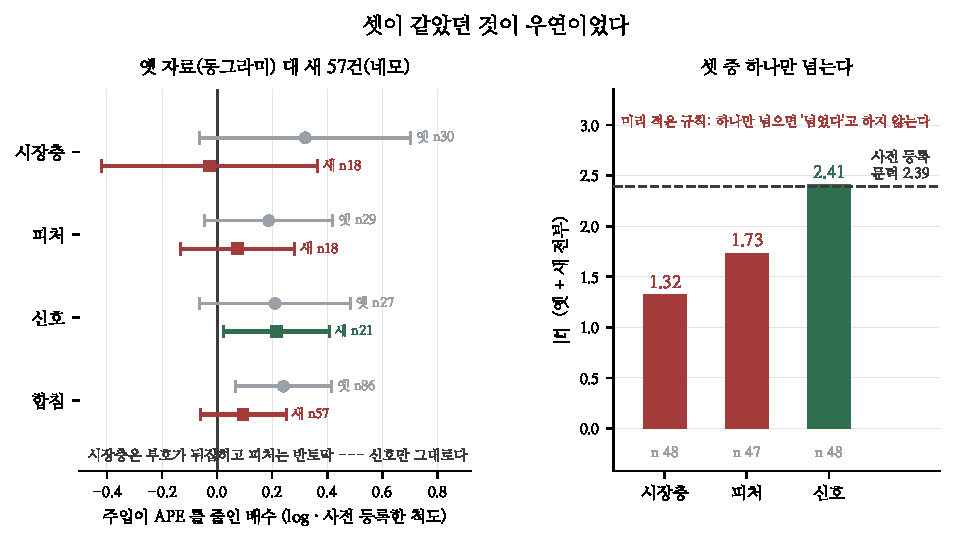
\includegraphics[width=\textwidth]{figs/replicate.pdf}
\caption{왼쪽 --- 옛 자료(동그라미)와 새 57건(네모)의 효과($\pm$1.96\,짝SE).
오른쪽 --- 전부 합쳐 사전 등록한 문턱과 견준 것.}
\end{figure*}

114회 예측을 돌리고 사전 등록한 척도로 읽었다.

\begin{center}\footnotesize
\begin{tabular}{lrrrrl}
\hline
& 전 & 후 & 효과 & 짝SE & $t$ \\
\hline
시장층 & 30 & 48 & $+$0.1899 & 0.1440 & $+$1.32 \\
피처 & 29 & 47 & $+$0.1442 & 0.0833 & $+$1.73 \\
\textbf{신호} & 27 & 48 & \textbf{$+$0.2130} & 0.0885 & \textbf{$+$2.41} \\
\hline
합침 & 86 & 143 & $+$0.1827 & 0.0626 & $+$2.92 \\
\hline
\end{tabular}
\end{center}

\textbf{신호만 2.39 를 넘는다.} 미리 적은 규칙대로 \textbf{``셋이 넘었다''고
하지 않는다.} 합침 $t{=}2.92$ 는 보조로만 적는다 --- 다만 이번에는 척도를
자료 보기 전에 고정했으므로 노트 295와 달리 척도 고르기가 아니다.

\paragraph{효과는 줄었다} 시장층 $+$0.3204 $\to$ $+$0.1899, 피처 $+$0.1874
$\to$ $+$0.1442. \textbf{승자의 저주다} --- 노트 295에서 ``필요 $n$ 은 관측된
효과에서 되짚은 값이라 낙관적''이라고 미리 적어 둔 그대로다. 되돌린 APE
감소도 21.4\% $\to$ \textbf{16.7\%} 다.

\section{진짜 수는 새 57건에 있다}

전과 후를 합치면 옛 자료가 섞여 복제인지 아닌지 안 보인다. \textbf{새로 더한
57건만} 떼어 봤다.

\begin{center}\footnotesize
\begin{tabular}{lrrlrr}
\hline
& \multicolumn{2}{c}{옛} & & \multicolumn{2}{c}{새} \\
& 효과 & $t$ & & 효과 & $t$ \\
\hline
시장층 & $+$0.3204 & $+$1.64 & & \textbf{$-$0.0275} & $-$0.14 \\
피처 & $+$0.1874 & $+$1.58 & & $+$0.0746 & $+$0.70 \\
\textbf{신호} & $+$0.2107 & $+$1.51 & & \textbf{$+$0.2160} & \textbf{$+$2.21} \\
\hline
합침 & $+$0.2411 & $+$2.69 & & $+$0.0945 & $+$1.19 \\
\hline
\end{tabular}
\end{center}

\begin{itemize}\itemsep2pt
\item \textbf{시장층은 부호가 뒤집혔다.} $+$0.3204 에서 $-$0.0275 다. 새
$n{=}18$ 에 짝SE 0.20 이라 ``나쁘다''고도 못 하지만, \textbf{$+$0.32 는
확실히 아니다.}
\item \textbf{피처는 반토막이다.} $+$0.1874 $\to$ $+$0.0746 (40\%).
\item \textbf{신호는 그대로다.} $+$0.2107 $\to$ $+$0.2160 --- 독립인 21건에서
\emph{같은 크기}가 다시 나오고 $t{=}2.21$ 이다.
\item \textbf{합침은 복제 안 된다.} $t{=}1.19$.
\end{itemize}

\paragraph{그러니 노트 295의 근거가 무너진다} 노트 295가 합치기를 정당화한
근거는 ``$t$ 가 1.64 · 1.58 · 1.51 로 거의 같다''였다. 새 자료에서는
\textbf{$+$2.21 · $+$0.70 · $-$0.14} 다. \textbf{그 일치 자체가 우연이었다} ---
$n{\approx}30$ 에 짝SE 0.12$\sim$0.20 인 셋의 $t$ 가 0.13 폭 안에 모이는 것은
신호가 아니라 요행이고, 나는 그 요행을 ``서로 안 겹치는 세 실험이 같은 말을
한다''로 읽었다.

\section{남은 것은 하나다}

\begin{center}\small
\begin{tabular}{lll}
\hline
층 & 판정 & 다음 \\
\hline
\textbf{신호} & \textbf{복제됨} & 왜 듣는지 갈라라 \\
피처 & 절반 · 미결 & 표본 더 \\
시장층 & 복제 안 됨 & 원래 수를 정정 \\
\hline
\end{tabular}
\end{center}

세 층을 한 덩어리로 ``주입''이라 부르면 $t{=}2.92$ 지만, \textbf{그 안에서
하나는 되고 하나는 부호가 뒤집힌다.} 합침은 ``무엇이든 넣으면 낫다''를
묻는 것이고, 그 물음은 \textbf{무엇을 넣을지 정해 주지 않는다.}

\paragraph{남은 것}
\begin{center}\small
\begin{tabular}{ll}
\hline
갈래 & 왜 \\
\hline
신호를 갈라라 & 어느 신호가 듣나 --- 아직 뭉치다 \\
시장층 정정 & 노트의 $+$0.32 를 새 수로 \\
피처 표본 더 & 남은 라벨 62건 \\
lab 회사 축 & 노트 294의 $+$0.0040 \\
\hline
\end{tabular}
\end{center}

\paragraph{규약} \textbf{일치를 증거로 쓰기 전에 그 일치를 복제하라.} 노트
295의 논증은 ``서로 독립인 셋이 같은 값을 낸다''였고 그것은 강한 논증
형식이다 --- \emph{일치가 진짜라면}. 각 $t$ 의 짝SE 가 자기 값만큼 컸으므로
0.13 폭의 일치는 애초에 우연으로 설명된다. \textbf{합침이 답한 물음과 내가
알고 싶던 물음이 달랐다} --- 나는 ``무엇을 넣을까''를 묻고 있었는데 합침은
``무엇이든 넣을까''에 답했다.

\end{document}
